\section{CTST - Lớp 10 - Ôn tập giữa học kì 1 - Đề 4}

\caulc

\Opensolutionfile{ans}[ans-ABCD]
%%%%%%=======Câu 1

\begin{ex}%[0D1N1-1]%[CTST - Lớp 10 - Ôn tập giữa học kì 1 - Đề 4]%[Phạm Hoài]
	Trong các câu sau, câu nào là không là một mệnh đề?
	\choice 
	{Số $5$ là số lẻ}
	{Số $\pi$ là một số hữu tỉ}
	{$2025-2024<3$}
	{\True Số $2\,025$ chia hết cho $5$ phải không?} 
	\loigiai{
		Số $2\,025$ chia hết cho $5$ phải không? không phải là mệnh đề.
	}
\end{ex}
%%%%%%=======Câu 2
\begin{ex} %[0D1N2-1]%[CTST - Lớp 10 - Ôn tập giữa học kì 1 - Đề 4]%[Phạm Hoài]
	Cho tập hợp $A=\{x \in \mathbb{N} \mid x \leq 5\}$. Số phần tử của tập hợp $A$ là
	\choice 
	{\True $6$}
	{$4$}
	{$3$}
	{$5$}
	\loigiai{
		Ta có $A=\{0 ; 1 ; 2 ; 3 ; 4 ; 5\}$.\\
		Vậy tập hợp $A$ có $6$ phần tử.
	}
\end{ex}
%%%%%%=======Câu 3
\begin{ex}%[0D2N1-2]%[CTST - Lớp 10 - Ôn tập giữa học kì 1 - Đề 4]%[Phạm Hoài]
	Cặp số nào sau đây là nghiệm của bất phương trình $2 x-3 y \leq 1$?
	\choice 
	{\True $(1;1)$}
	{$(2;0)$}
	{$(3;1)$}
	{$(2;-1)$}
	\loigiai{
		Thay các cặp số vào bất phương trình $2 x-3 y \leq 1$ ta thấy cặp số $(1 ; 1)$ thỏa mãn.
	}
\end{ex}
%%%%%%=======Câu 4
\begin{ex}%[0D3N1-5]%[CTST - Lớp 10 - Ôn tập giữa học kì 1 - Đề 4]%[Phạm Hoài]
\immini{Cho hàm số $y=f(x)$ có đồ thị như hình bên. Khẳng định nào sau đây đúng
	\choice
	{ Hàm số $y=f(x)$ đồng biến trên khoảng $(-\infty ;-2)$}
	{Hàm số $y=f(x)$ đồng biến trên khoảng $(2 ;+\infty)$}
	{ Hàm số $y=f(x)$ đồng biến trên khoảng $(-2 ; 2)$}
	{\True Hàm số $y=f(x)$ đồng biến trên khoảng $(-2 ; 0)$}}
	{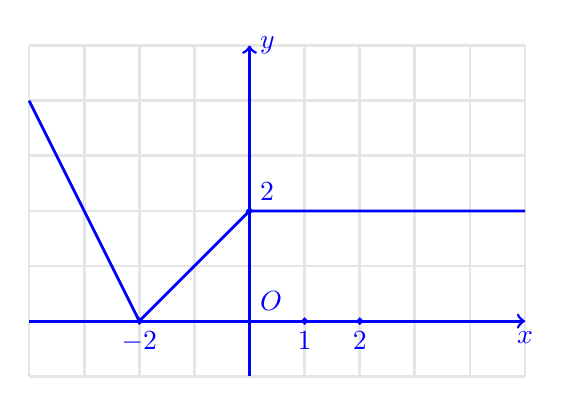
\begin{tikzpicture}[scale=0.7,line width=1pt,blue]
		%	\path (0,0)node{\includegraphics[scale=1]{Nguoi1.png}};
			\draw[gray!20] (-4,-1)grid(5,5);
			\draw[->] (-4,0)--(0,0)node[above right]{$O$}--(5,0)node[below]{$x$};
			\draw[->] (0,-1)--(0,5)node[right]{$y$};
			\draw (-4,4)--(-2,0)circle(1pt)node[below]{$-2$}--(0,2)circle(1pt)node[above right]{$2$}--(5,2);
			\draw (1,0)circle(1pt)node[below]{$1$}(2,0)circle(1pt)node[below]{$2$};
	\end{tikzpicture}}
	\loigiai{
		Dựa vào đồ thị, hàm số $y=f(x)$ đồng biến trên khoảng $(-2 ; 0)$.
	}
\end{ex}
%%%%%%=======Câu 5
\begin{ex}%[0D3H2-1]%[CTST - Lớp 10 - Ôn tập giữa học kì 1 - Đề 4]%[Phạm Hoài]
	Trục đối xứng của parabol $y=-x^2+5 x+3$ là đường thẳng có phương trình
	\choice
	{$x=\dfrac{5}{4}$}
	{$x=-\dfrac{5}{2}$}
	{$x=-\dfrac{5}{4}$}
	{\True $x=\dfrac{5}{2}$}
	\loigiai{
		Trục đối xứng của parabol $y=a x^2+b x+c$ là đường thẳng $x=-\dfrac{b}{2 a}$.\\
		Trục đối xứng của parabol $y=-x^2+5 x+3$ là đường thẳng $x=\dfrac{5}{2}$.
	}
\end{ex}
%%%%%%=======Câu 6
\begin{ex} %[0D1N1-4]%[CTST - Lớp 10 - Ôn tập giữa học kì 1 - Đề 4]%[Phạm Hoài]
	Cách phát biểu nào sau đây không thể dùng để phát biểu mệnh đề $A \Rightarrow B$.
	\choice
	{Nếu $A$ thì $B$}
	{\True $A$ là điều kiện cần đề có $B$}
	{$A$ kéo theo $B$}
	{$A$ là điều kiện đủ để có $B$}
	\loigiai{$A\Rightarrow B$ được phát biểu là 
	\begin{itemize}
		\item Nếu $A$ thì $B$.
		\item $A$ kéo theo $B$.
		\item $A$ là điều kiện đủ để có $B$.
		\end{itemize}
	Do đó $A$ là điều kiện cần để có $B$ không thể dùng để phát biểu mệnh đề $A\Rightarrow B$.}
\end{ex}
%%%%%%=======Câu 7
\begin{ex}%[0D1N3-1]%[CTST - Lớp 10 - Ôn tập giữa học kì 1 - Đề 4]%[Phạm Hoài]
	Cho hai tập hợp $A=\{0 ; 2 ;-6 ; 4\}$ và $A=\{0 ; 6 ;-7 ;-5 ;-2\}$. Tìm tập hợp $A \cap B=$?
	\choice
	{$\{2 ;-6 ; 4\}$}
	{$\{-7 ;-5 ; 6 ;-2\}$}
	{\True $\{0\}$}
	{$\{0 ; 2 ; 4 ; 6 ;-7 ;-6 ;-5 ;-2\}$}
	\loigiai{
		Tập hợp $A \cap B=\{0\}$ vì chỉ có $0$ vừa thuộc tập $A$ vừa thuộc tập $B$.
	}
\end{ex}
%%%%%%=======Câu 8
\begin{ex}%[0D2N2-2]%[CTST - Lớp 10 - Ôn tập giữa học kì 1 - Đề 4]%[Phạm Hoài]
	Cặp số nào sau đây là nghiệm của hệ bất phương trình $\heva{&2 x+3 y+3 \leq 0 \\& 3 x+3 y-2 \leq 0}$?
	\choice 
	{$(1;2)$}
	{$(-1;1)$}
	{$(3;-1)$}
	{\True $(-1;-2)$}
	\loigiai{
		Thay các cặp số lần lượt vào các bất phương trình ta thấy cặp $(-1 ;-2)$ thỏa mãn cả hai bất phương trình đã cho.
	}
\end{ex}
%%%%%%=======Câu 9
\begin{ex}%[0D3H1-2]%[CTST - Lớp 10 - Ôn tập giữa học kì 1 - Đề 4]%[Phạm Hoài]
	Tìm tập xác định của hàm số $y=\dfrac{6-4 x}{\sqrt{2-x}}$.
	\choice 
	{ $\mathscr{D}=\mathbb{R} \setminus\{2\}$}
	{\True $\mathscr{D}=(-\infty ; 2)$}
	{$\mathscr{D}=(-\infty ; 2]$}
	{$\mathscr{D}=(2 ;+\infty)$}
	\loigiai{
		Hàm số xác định khi $2-x>0 \Leftrightarrow x<2$.\\
		 Do đó tập xasd định $\mathscr{D}=(-\infty;2)$.
	}
\end{ex}
%%%%%%=======Câu 10
\begin{ex}%[0D2V2-2]%[CTST - Lớp 10 - Ôn tập giữa học kì 1 - Đề 4]%[Phạm Hoài]
 Các số $x$ và $y$ thỏa mãn hệ bất phương trình $\heva{&0 \leq y \leq 4 \\& x \geq 0 \\& x-y-1 \leq 0 \\& x+2 y-10 \leq 0}$. Giá trị lớn nhất của biết thức $F(x ; y)=7 x+10 y+2024$ là
	\choice 
	{$2\,024$}
	{$2\,078$}
	{\True $2\,082$}
	{$2\,064$}
	\loigiai{
		Vẽ đường thẳng $d_1\colon x-y-1=0$, đường thẳng $d_1$ qua hai điểm $(0 ;-1)$ và $(1 ; 0)$.\\
		Vẽ đường thẳng $d_2\colon  x+2 y-10=0$, đường thẳng $d_2$ qua hai điểm $(0 ; 5)$ và $(2 ; 4)$.\\
		Vẽ đường thẳng $d_3\colon y=4$.
		\begin{center}
			\begin{tikzpicture}[line width=1pt,blue]
				%	\path (0,0)node{\includegraphics[scale=1]{Nguoi1.png}};
				\draw[gray!20] (-1,-1.5)grid(5,5);
				\draw[->] (-1,0)--(0,0)node[above right]{$O$}--(5,0)node[below]{$x$};
				\draw[->] (0,-1.5)--(0,5)node[right]{$y$};
				\draw (-1,-2)--(5,4)(-1,5.5)--(5,2.5) (-1,4)--(5,4); 
				\path[pattern=north east lines] (-1,4)--(-1,5)--(5,5)--(5,4)--cycle ;
				\path[pattern=north east lines] (-1,5.5)--(5,5.5)--(5,2.5)--cycle ;
				\path[pattern=north east lines] (-1,-2)--(5,-2)--(5,4)--cycle ;
				\path[pattern=north east lines] (-1,-2)--(0,-2)--(0,5.5)--(-1,5.5)--cycle ;
				\path[pattern=north east lines] (-1,-2)--(-1,0)--(5,0)--(5,-2)--cycle ;
				\draw (0,4)circle(1pt)node[above left]{$4$}
				(0,4)circle(1pt)node[below right]{$C$}(2,4)circle(1pt)node[above]{$B$}(4,3)circle(1pt)node[above]{$A$}(1,0)circle(1pt)node[above]{$E$}(1,0)circle(1pt)node[below]{$1$}(2,0)circle(1pt)node[below]{$2$}(4,0)circle(1pt)node[below]{$4$};
			\end{tikzpicture}
		\end{center}
		Miền nghiệm của hệ bất phương trình là miền ngũ giác $A B C O E$ với
		$A(4;3)$; $B(2;4)$; $C(0;4)$; $E(1; 0)$.\\
		Ta có $F(4; 3)=2\,082$, $F(2;4)=2\,078$, $F(0;4)=2\,064$, $F(1; 0)=2\,031$, $F(0; 0)=2\,024$.\\
		Vậy giá trị lớn nhất của biết thức $F(x ; y)=7 x+10 y+2\,024$ bằng $2\,082$ khi $x=3$; $y=4$.
	}
\end{ex}
%%%%%%=======Câu 11
\begin{ex}%[0D3V2-1]%[CTST - Lớp 10 - Ôn tập giữa học kì 1 - Đề 4]%[Phạm Hoài]
	 Biết rằng đồ thị hàm số $(P): y=a x^2+b x+c$ có đỉnh $I(2 ;-5)$ và cắt trục tung tại điểm có tung độ bằng $-1$. Khi đó $S=a+b+c$ là
	\choice
	{\True $S=-4$}
	{$S=4$}
	{$S=-2$}
	{$S=2$}
	\loigiai{
		Vì $(P)$ cắt trục tung tại điểm có tung độ bằng $-1$ nên $(P)$ đi qua điểm $(0 ;-1)$ nên $c=-1$.\\
		Vì $(P)$ có đỉnh $I(2 ;-5)$ nên 
		\begin{eqnarray*}
		\heva{&a \cdot 2^2+b \cdot 2+c=-5 \\& \dfrac{-b}{2 a}=2}& \Rightarrow &\heva{&4 a+2 b-1=-5 \\& -b=4 a}\\
		 &\Rightarrow &\heva{&4 a+2 b=-4 \\& 4 a+b=0}\\
		 & \Rightarrow &\heva{&a=1 \\& b=-4.}
		\end{eqnarray*}
		Vậy $S=a+b+c=1+(-4)+(-1)=-4$.
	}
\end{ex}
%%%%%%=======Câu 12
\begin{ex}%[0D1V3-5]%[CTST - Lớp 10 - Ôn tập giữa học kì 1 - Đề 4]%[Phạm Hoài]
	 Trong lớp 10C có $45$ học sinh trong đó có $25$ em thích môn Văn, $20$ em thích môn Toán, $18$ em thích môn Sử, $6$ em không thích môn nào, $5$ em thích cả ba môn. Hỏi số em thích chỉ một môn trong ba môn trên.
	\choice 
	{$15$}
	{\True $20$}
	{$25$}
	{$30$}
	\loigiai{
		Gọi $a$, $b$, $c$ theo thứ tự là số học sinh chỉ thích môn Văn, Sử, Toán;\\
		$x$ là số học sinh chỉ thích hai môn là Văn và Toán.\\
		$y$ là số học sinh chỉ thích hai môn là Sử và Toán.\\
		$z$ là số học sinh chỉ thích hai môn là Văn và Sử.\\
		Do có $6$ em không thích môn nào nên số em thích ít nhất một môn là $45-6=39$.\\
		Dựa vào biểu đồ Ven ta có hệ phương trình
		\begin{center}
			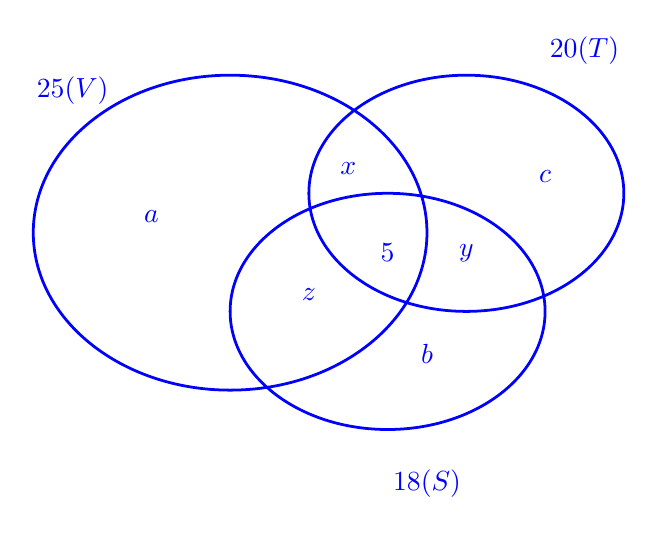
\begin{tikzpicture}[line width=1pt,blue]
				%	\path (0,0)node{\includegraphics[scale=1]{Nguoi1.png}};
			%	\draw[gray!20] (-3,-1.5)grid(5,5);
			%	\draw[->] (-1,0)--(0,0)node[above right]{$O$}--(5,0)node[below]{$x$};
			%	\draw[->] (0,-1.5)--(0,5)node[right]{$y$};
				\draw (-2.5,2.5) arc(180:0:2.5 and 2) (-2.5,2.5) arc(180:360:2.5 and 2)
				(1,3) arc(180:0:2 and 1.5) (1,3) arc(180:360:2 and 1.5)
				(0,1.5) arc(180:0:2 and 1.5) (0,1.5) arc(180:360:2 and 1.5)
				;
				\path (-1,2.5)node[above]{$a$}(1,1.5)node[above]{$z$}(2.5,0.7)node[above]{$b$}(3,2)node[above]{$y$}(4,3)node[above]{$c$}(2,2)node[above]{$5$}(1.5,3.1)node[above]{$x$}(-2,4)node[above]{$25(V)$} (4.5,4.5)node[above]{$20(T)$}(2.5,-1)node[above]{$18(S)$};
		
			\end{tikzpicture}
		\end{center}
		$\heva{&a+x+z+5=25 \, \quad (1)\\&b+y+z+5=18\, \quad (2) \\&c+x+y+5=20\, \quad (3) \\&	x+y+z+a+b+c+5=39.\, \quad (4)}$\\
		Cộng vế với vế $(1)$, ($2)$, $(3)$ ta có
		$a+b+c+2(x+y+z)+15=63\, \quad (5)$.\\
		Từ $(4)$ và $(5)$ ta có
		$ a+b+c+2(39-5-a-b-c)+15=63 \Leftrightarrow a+b+c=20$.\\
		Vậy chỉ có $20$ em thích chỉ một môn trong ba môn trên.
	}
\end{ex}
\Closesolutionfile{ans}

\indapan{6}{ans-ABCD}

\cauds

\Opensolutionfile{ans}[ans-DS]
%%%%%%=======Câu 1
\begin{ex}%[0D1H3-4]%[CTST - Lớp 10 - Ôn tập giữa học kì 1 - Đề 4]%[Phạm Hoài]
	Cho ba tập hợp $A=(-2 ; 4]$, $B=(1 ;+\infty)$ và $C=[-5 ; m-3]$ ($C \neq \varnothing$). Xét tính đúng sai của các mệnh đề sau?
	\choiceTF
	{\True $A \cap B=(1 ; 4]$}
	{\True $A \cup B=(-2 ;+\infty)$}
	{$A \setminus B=(-2 ; 1)$}
	{\True Có $6$ giá trị nguyên của $m$ đề $B \cap C=\varnothing$}
	\loigiai{
		\begin{itemchoice}
			\itemch \textbf{Đúng}. \\Ta có $A \cap B=(1 ; 4]$.
				\begin{center}
				\begin{tikzpicture}[line width=1pt,blue]
				\draw[->] (-5,0)--(5,0);
				\draw (-2,-0.3)node[below]{$-2$}(1,-0.3)node[below]{$1$}(4,-0.3)node[below]{$4$} 
					(-2,0)node[]{$\left(\right.$}(1,0)node[]{$\left(\right.$}(4,0)node[]{$\left.\right]$};
				\path[pattern=north east lines](-5,-0.2)--(-5,0.2)--(-2,0.2)--(-2,-0.2)--cycle;	
				\path[pattern=north west lines](-5,-0.2)--(-5,0.3)--(1,0.2)--(1,-0.2)--cycle;
				\path[pattern=north west lines](4,-0.2)--(4,0.2)--(5,0.2)--(5,-0.2)--cycle;	
				\end{tikzpicture}
			\end{center}
			\itemch \textbf{Đúng}.\\Ta có $A \cup B=(-2 ;+\infty)$.
				\begin{center}
				\begin{tikzpicture}[line width=1pt,blue]
					\draw[->] (-5,0)--(5,0);
					\draw (-2,-0.3)node[below]{$-2$}(1,-0.3)node[below]{$1$}(4,-0.3)node[below]{$4$} 
					(-2,0)node[]{$\left(\right.$}(1,0)node[]{$\left(\right.$}(4,0)node[]{$\left.\right]$};
					\path[pattern=north east lines](-5,-0.2)--(-5,0.2)--(-2,0.2)--(-2,-0.2)--cycle;	
				\end{tikzpicture}
			\end{center}
			\itemch \textbf{Sai}.\\ Ta có: $A \setminus B=(-2 ; 1]$.
				\begin{center}
				\begin{tikzpicture}[line width=1pt,blue]
						\draw[->] (-5,0)--(5,0);
					\draw (-2,-0.3)node[below]{$-2$}(1,-0.3)node[below]{$1$}(4,-0.3)node[below]{$4$} 
					(-2,0)node[]{$\left(\right.$}(1,0)node[]{$\left(\right.$}(4,0)node[]{$\left.\right]$};
					\path[pattern=north east lines](-5,-0.2)--(-5,0.2)--(-2,0.2)--(-2,-0.2)--cycle;	
					\path[pattern=north east lines](1,-0.2)--(1,0.3)--(5,0.2)--(5,-0.2)--cycle;
					\path[pattern=north west lines](4,-0.2)--(4,0.2)--(5,0.2)--(5,-0.2)--cycle;	
				\end{tikzpicture}
			\end{center}
			\itemch \textbf{Đúng}.\\ $B \cap C=\varnothing$ khi $\heva{&m-3>-5 \\& m-3 \leq 1}\Leftrightarrow \heva{&m>-2 \\& m \leq 4}\Leftrightarrow-2<m \leq 4$.\\
			Vì $m$ là số nguyên nên $m \in\{-1 ; 0 ; \ldots ; 4\}$. \\
			Vậy có $6$ giá trị nguyên của $m$ để $B \cap C= \varnothing $.
				\begin{center}
				\begin{tikzpicture}[line width=1pt,blue]
					\draw[->] (-5,0)--(5,0);
					\draw (-2,-0.3)node[below]{$-5$}(1,-0.3)node[below]{$m-3$}(2,-0.3)node[below]{$1$} 
					(-2,0)node[]{$\left[\right.$}(1,0)node[]{$\left.\right]$}(2,0)node[]{$\left(\right.$};
					\path[pattern=north east lines](-5,-0.2)--(-5,0.2)--(2,0.2)--(2,-0.2)--cycle;	
					\end{tikzpicture}
			\end{center}
		\end{itemchoice}	
	}
\end{ex}
%%%%%%=======Câu 2
\begin{ex}%[0D1C3-5]%[CTST - Lớp 10 - Ôn tập giữa học kì 1 - Đề 4]%[Phạm Hoài]
	 Một lớp học có $32$ học sinh trong đó gồm có $5$ học sinh giỏi cả hai môn Văn và Toán, $13$ học sinh không giỏi môn nào trong cả hai môn Văn và Toán, số học sinh giỏi Toán bằng hai lần số học sinh giỏi Văn.
	\choiceTF
	{Số học sinh giỏi cả Văn và Toán lớn hơn số học sinh không giỏi môn nào trong cả hai môn Văn và Toán}
	{\True Nếu gọi $x$ là số học sinh chỉ giỏi Toán và $y$ là số học sinh chỉ giỏi Văn thì $x+y=14$}
	{\True Nếu gọi $x$ là số học sinh chỉ giỏi Toán và $y$ là số học sinh chỉ giỏi Văn thì $x-2 y=5$}
	{Số học sinh chỉ giỏi Toán là $12$}
	\loigiai{
			\begin{center}
			\begin{tikzpicture}[line width=1pt,blue]
				\draw (-2.5,1.5) arc(180:0:4 and 3) (-2.5,1.5) arc(180:360:4 and 3)
				(-1,3)..controls++(10:1.5) and++(55:1.5)..(1,0)..controls++(-150:1.5)and++(-150:1.5)..(-1,3) ;	
				\draw (0,1.5)..controls++(90:1.5) and++(90:1.5)..(3,1.7)..controls++(-90:1.5)and++(-90:1.5)..(0,1.5) ;	
				\path (-1.4,2)node[right]{$\text{Toán}$}(1.5,1.5)node[above]{$\text{Văn}$}(0.5,1)node[above]{$5$}(1.5,-0.5)node[above]{$13$};
				
			\end{tikzpicture}
		\end{center}
		\begin{itemchoice}
			\itemch \textbf{Sai}.\\ Số học sinh giỏi cả Văn và Toán là $5$, số học sinh không giỏi môn nào trong cả hai môn Văn và Toán là $13 $nên $5<13$.
			\itemch \textbf{Đúng}.\\ Ta có $x+y+5+13=32 \Leftrightarrow x+y=14$.
			\itemch \textbf{Đúng}.\\ Ta có $x+5=2(y+5) \Leftrightarrow x-2 y=5$.
			\itemch \textbf{Sai}.\\ Ta có $\heva{&x+y=14 \\& x-2 y=5}\Leftrightarrow\heva{&x=11 \\& y=3}$ nên số học sinh chỉ giỏi Toán là $11$.
		\end{itemchoice}
	}
\end{ex}
%%%%%%=======Câu 3
\begin{ex} %[0D2V2-3]%[CTST - Lớp 10 - Ôn tập giữa học kì 1 - Đề 4]%[Phạm Hoài]
	Một cơ sở sản xuất dự định dùng hai loại nguyên liệu để chiết suất ít nhất $140$ kg chất A và ít nhất $9$ kg chất B. Từ mỗi tấn nguyên liệu loại $\text{I}$ giá $4{,}5$ triệu đồng, có thể chiết suất được $20$ kg chất A và $0{,}6$ kg chất B. Từ mỗi tấn nguyên liệu loại $\text{II}$ giá $3{,}5$ triều đồng, có thể chiết suất được $10$ kg chất A và $1{,}5$ kg chất B. Biết cơ sở cung cấp nguyên liệu chỉ cung cấp không quá $10$ tấn nguyên liệu loại $\text{I}$ và không quá $9$ tấn nguyên liệu loại $\text{II}$. Giả sử cơ sở sản xuất đó dùng $x$ tấn nguyên liệu loại $\text{I}$ và $y$ tấn nguyên liệu loại $\text{II}$ để sản xuất. Từ các dữ kiện đã có, xác định tính đúng sai của các mệnh đề sau
	\choiceTF
	{Điều kiện của biến $x$ là $0 \leq x \leq 9$}
	{\True Số tiền mà cơ sở sản xuất phải trả để mua nguyên liệu là $4{,}5 x+3{,}5 y$ (triệu)}
	{Số tiền ít nhất mà cơ sở đó phải trả để mua nguyên liệu là $35{,}6$ (triệu)}
	{\True Để số tiền mua nguyên liệu ít nhất cơ sở đó dùng $a$ tấn nguyên liệu loại $\text{I}$ và $b$ tấn nguyên liệu loại $\text{II}$. Khi đó $a+b=9$}
	\loigiai{
		
		Theo bài ra ta có hệ bất phương trình $\heva{&0 \leq x \leq 10 \\& 0 \leq y \leq 9 \\& 20 x+10 y \geq 140 \\& 0{,}6 x+1{,}5 y \geq 9.}$\\
		Số tiền mà cơ sở phải trả để mua nguyên liệu là $T=4{,}5 x+3{,}5 y$.\\
		Ta có miền nghiệm là hình tứ giác $A B C D$ (như hình vẽ). 
			\begin{center}
			\begin{tikzpicture}[line width=1pt,blue]
				%	\path (0,0)node{\includegraphics[scale=1]{Nguoi1.png}};
				\draw[gray!20] (-2,-1)grid(12,10);
				\draw[->] (-2,0)--(0,0)node[above right]{$O$}--(12,0)node[below]{$x$};
				\draw[->] (0,-1)--(0,10)node[right]{$y$};
				\clip(-2,-1) rectangle (12,10);
				\draw (-2,18)--(12,-10)(-2,6.8)--(12,1.2) (-2,9)--(12,9) (10,-1)--(10,10); 
				\path[pattern=north east lines] (-2,-1)--(-2,11)--(2,10)--(7.5,-1)--cycle ;
				\path[pattern=north west lines] (-2,9)--(-2,10)--(12,10)--(12,9)--cycle ;
				\path[pattern=north east lines] (10,10)--(12,10)--(12,-1)--(10,-1)--cycle ;
				\path[pattern=north east lines] (-2,6.8)--(-2,-1)--(10,-1)--(12,1.2)--cycle ;
				\draw (2.5,9)circle(1pt)node[above right]{$A$}
				(10,9)circle(1pt)node[below left]{$B$}(10,2)circle(1pt)node[above right]{$C$}(5,4)circle(1pt)node[below left]{$D$}(0,6)circle(1pt)node[below left]{$6$}(7,0)circle(1pt)node[below left]{$7$}(10,0)circle(1pt)node[below left]{$10$};
			\end{tikzpicture}
		\end{center}
		Trong đó:
		Toạ độ của điểm $A$ là nghiệm của hệ $\heva{&y=9 \\& 2 x+y=14}\Leftrightarrow\heva{&x=2{,}5 \\&y=9} \Rightarrow A(2{,}5; 9)$.\\
		$B(10; 9)$.\\
		Toạ độ của điểm $C$ là nghiệm của hệ $\heva{&x=10 \\& 0{,}6 x+1{,}5 y=9}\Leftrightarrow\heva{&x=10 \\& y=2}\Rightarrow C(10 ; 2)$.\\
		Toạ độ của điểm $D$ là nghiệm của hệ $\heva{&0{,}6 x+1{,}5 y=9 \\& 2 x+y=14}\Leftrightarrow \heva{&x=5 \\& y=4} \Rightarrow D(5 ; 4)$.\\
		Ta có $T(2{,}5; 9)=4{,}5\cdot 2{,}5+3{,}5\cdot 9=42{,}75$; $T(10; 9)=76{,}5$, $T(10; 2)=52$, $T(5; 4)=36{}5$.\\
		Vậy $\min T=36{,}5 \Leftrightarrow (x, y)=54$.
		\begin{itemchoice}
			\itemch \textbf{Sai}.
			\itemch \textbf{Đúng}.
			\itemch \textbf{Sai}.
			\itemch \textbf{Đúng}.
		\end{itemchoice}
	}
\end{ex}
%%%%%%=======Câu 4
\begin{ex}%[0D3V2-2]%[CTST - Lớp 10 - Ôn tập giữa học kì 1 - Đề 4]%[Phạm Hoài]
	 Cho hàm số $f(x)=\heva{&-x^2-6 a x+5 & \text { khi } x<0 \\& \sqrt{x+2} & \text { khi } x \geq 0}$, $a$ là tham số.
	\choiceTF
	{\True Đồ thị hàm số đi qua điểm $M(2; 2)$}	
	{Với $a=1$, hàm số nghịch biến trên khoảng $(-\infty ;-3)$}
	{Tập xác định của hàm số là $[-2 ;+\infty)$}
	{\True Giá trị lớn nhất của hàm số trên khoảng $(-10 ; 0)$ bằng 41 khi $a=2$}
	\loigiai{
		\begin{itemchoice}
			\itemch \textbf{Đúng}.\\ Với $x=2>0$ ta có $f(x)=\sqrt{x+2}$. Suy ra $f(2)=\sqrt{2+2}=2$.\\
			Do đó đồ thị hàm số đi qua điểm $M(2 ; 2)$.
			\itemch \textbf{Sai}.\\ Khi $a=1$, trên khoảng $(-\infty ;-3)$ ta có $f(x)=-x^2-6 a x+5=-x^2-6 x+5$ là hàm số bậc 2 có tọa độ đỉnh $I(-3 ; 14)$. Suy ra hàm số đồng biến trên khoảng $(-\infty ;-3)$.
			\itemch \textbf{Sai}.\\ Với $x<0$ hàm số $f(x)=-x^2-6 a x+5$ xác định.\\
			Với $x \geq 0$ hàm số $f(x)=\sqrt{x+2}$ xác định.\\
			Suy ra hàm số $f(x)$ xác định trên $\mathbb{R}$ hay tập xác định $\mathscr{D}=\mathbb{R}$.
			\itemch \textbf{Đúng}.\\ Trên khoảng $(-10 ; 0)$ hàm số $f(x)=-x^2-6 a x+5$.\\
			Hàm số đạt giá trị lớn nhất tại $x=-3 a$.\\
			Ta có: $\heva{&f(-3 a)=41 \\& -10<-3 a<0} \Leftrightarrow\heva{&9 a^2+5=41 \\& 0<a<\dfrac{10}{3}} \Leftrightarrow a=2$.
		\end{itemchoice}
	}
\end{ex}
\Closesolutionfile{ans}

\indapan{3}{ans-DS}

\caukq

\Opensolutionfile{ans}[ans-KQ]
%%%%%%=======Câu 1
\begin{ex}%[0D1H1-2]%[CTST - Lớp 10 - Ôn tập giữa học kì 1 - Đề 4]%[Phạm Hoài]
	Tìm giá trị của số $x$ để câu \lq \lq Tổng của số $4$ và $x$ là $15$\rq \rq \, là một mệnh đề đúng.
	\shortans{11}
	\loigiai{
		Ta có $4+x=15\Rightarrow x=11$.
	}
\end{ex}
%%%%%%=======Câu 2
\begin{ex} %[0D2N1-2]%[CTST - Lớp 10 - Ôn tập giữa học kì 1 - Đề 4]%[Phạm Hoài]
	Tìm số nguyên dương $y_0$ để cặp số $\left(1{,}5 ; y_0\right)$ là một nghiệm của bất phương trình $6 x-y>7{,}5$.
	\shortans{1}
	\loigiai{ 
		$6\cdot 1{,}5-y_0>7{,}5\Leftrightarrow y_0<9-7{,}5=1{,}5$.\\
		Vì $y_0$ nguyên dương nên $y_0=1$.
	}
\end{ex}
%%%%%%=======Câu 3
\begin{ex}%[0D3H1-3]%[CTST - Lớp 10 - Ôn tập giữa học kì 1 - Đề 4]%[Phạm Hoài]
	Tập giá trị của hàm số $y=\sqrt{x^2-4 x+13}$ được viết dưới dạng $[a ;+\infty)$. Tìm $a$.
	\shortans{3}
	\loigiai{
		\begin{itemize}
			\item Điều kiện xác định: $x^2-4 x+13 \geq 0 \Leftrightarrow(x-2)^2+9 \geq 0$ đúng $\forall x \in \mathbb{R}$.\\
			Tập xác định: $\mathscr{D}=\mathbb{R}$.\\
			\item Ta có $x^2-4 x+13=(x-2)^2+9 \geq 9 \Leftrightarrow \sqrt{(x-2)^2+9} \geq 3$.\\
			Tập giá trị của hàm số đã cho là $[3 ;+\infty)$.\\
			Vậy $a=3$.
		\end{itemize}
	}
\end{ex}
%%%%%%=======Câu 4
\begin{ex}%[0D3V2-1]%[CTST - Lớp 10 - Ôn tập giữa học kì 1 - Đề 4]%[Phạm Hoài]
	Đồ thị hàm số bậc hai $y=a x^2+b x+c$ có đỉnh là $I(1 ;-2)$ và đi qua điểm $A(2 ;-3)$. Khi đó, $a+2 b-c$ bằng bao nhiêu?
	\shortans{6}
	\loigiai{
		Đồ thị hàm số bậc hai $y=a x^2+b x+c$ có đỉnh $I\left(-\dfrac{b}{2 a} ;-\dfrac{\Delta}{4 a}\right)$ nên có $\heva{&-\dfrac{b}{2 a}=1 \\& a \cdot 1+b \cdot 1+c=-2.}$\\
		Đồ thị hàm số $y=a x^2+b x+c$ đi qua điểm $A(2 ;-3)$ nên $4 a+2 b+c=-3$.\\
		Do đó: $\heva{&-\dfrac{b}{2 a}=1 \\& a+b+c=-2 \\& 4 a+2 b+c=-3} \Leftrightarrow\heva{&a=-1 \\& b=2 \\& c=-3.}$\\
		Vậy $a+2 b-c=-1+2 \cdot 2+3=6$.
	}
\end{ex}
%%%%%%=======Câu 5
\begin{ex} %[0D1V3-3]%[CTST - Lớp 10 - Ôn tập giữa học kì 1 - Đề 4]%[Phạm Hoài]
	Cho tập hợp $A=[-2 ; 3]$ và tập hợp $B=\left[\dfrac{m-1}{3};+\infty\right)$. Tổng tất cả các giá trị nguyên của tham số $m$ để $A \cap B$ có đúng ba phần tử là số nguyên là?
	\shortans{9}
	\loigiai{
		Ta có: Để $A \cap B$ có đúng ba phần tử là số nguyên thì $A \cap B$ chứa $3$ phần tử $1$; $2$; $3$ nên
		\\$
		\heva{&\dfrac {m - 1}{3} \leq 1\\&\dfrac{m - 1}{3} > 0} \Leftrightarrow \heva{&m \leq 4 \\&	m>1} \Leftrightarrow 1<m \leq 4.$\\
		Mà $m \in \mathbb{Z} \Rightarrow m \in\{2 ; 3 ; 4\}$.\\
		Vậy tổng tất cả các giá trị nguyên của tham số $m$ để $A \cap B$ có đúng ba phần tử là số nguyên $2+3+4=9$.
	}
\end{ex}
%%%%%%=======Câu 6
\begin{ex}%[0D3C2-6]%[CTST - Lớp 10 - Ôn tập giữa học kì 1 - Đề 4]%[Phạm Hoài]
	\immini{ Một miếng nhôm có bề ngang $32$ cm được uốn cong tạo thành rảnh dẫn nước bằng chia tấm nhôm thành $3$ phần rồi gấp $2$ bên lại theo một góc vuông. Người ta cần nghiên cứu cách để tạo ra đường rảnh có diện tích mặt cắt ngang $S$ lớn nhất để có thể cho nước đi qua nhiều nhất. Tích bề ngang của ba phần là bao nhiêu để có được diện tích $S$ lớn nhất.
	\shortans{1\,024}}
	{	\begin{tikzpicture}[blue]
			\draw (0.5,0.7)--(-2.5,0.7)--(-4.3,-1.5)--(-0.85,-1.5)--cycle (-0.3,0.7)--(-1.73,-1.5)(-1.6,0.7)--(-3.3,-1.5);
			\draw[<->] (-4.3,-2)--(-0.85,-2)node[pos=0.5,below]{$32$ cm};
			\draw(-4.3,-2.1)--(-4.3,-1.9)(-0.85,-2.1)--(-0.85,-1.9);
			\draw[<->] (-1.6,1)--(-2.5,1)node[pos=0.5,above]{$x$ cm};
			\draw(-1.6,1.1)--(-1.6,0.9)(-2.5,1.1)--(-2.5,0.9);
			\draw (2.35,0.8)--(1.43,0.8)--(1.4,1.5)--(0.16,-0.5)--(0.16,-1.4)--(1.73,-1.35)--(1.73,-0.5)--(2.7,1.5)--(2.7,0.8)--(1.73,-1.35)(1.43,0.8)--(0.16,-1.4)
			(0.7,0.38)--(0.7,-0.45)--(2.15,-0.45)--(2.15,0.38)--cycle;
			\draw[<->] (0.7,0.6)--(2.15,0.6);
			\draw(0.7,0.5)--(0.7,0.7)(2.15,0.5)--(2.15,0.7);
			\draw [<-](1.5,0.6)--(2,1.7)node[above]{$(32-2x)$ cm};
			\draw[<->] (2.3,-0.45)--(2.3,0.38)node[pos=0.5,right]{$x$ cm};
			\draw(2.2,-0.45)--(2.4,-0.45)(2.2,0.38)--(2.4,0.38);
			\draw [<-](1.5,0)--(2.3,-.7)node[below right]{Mặt cắt};
	\end{tikzpicture}}
	\loigiai{ Gọi $x$ là bề ngang hai phần bên của tấm nhôm $(0 \leq x \leq 16)$.\\
		Diện tích mặt ngang $S=(32-2 x) x=-2 x^2+32 x$.\\
		\begin{center}
			
\begin{tikzpicture}[font=\normalsize,t style/.style={style=solid}]
				%dòng khai báo
				\tkzTabInit[nocadre=true,lgt=4,espcl=2.5,deltacl=0.5]
				{$x$ /0.75, $S(x)=-2x^2+32x$/2}
				{$ 0 $,$ 8 $,$ 16 $}
				%dòng biến thiên
				\tkzTabVar{-/$0$,+/$128$,-/$0$} %+ hoac-
			\end{tikzpicture}
		\end{center}
		Để nước đi qua nhiều nhất thì diện tích mặt cắt ngang của rảnh là lớn nhất $S=128$ tại $x=8$.\\
		Vậy cần chia tấm nhôm ra ba phần là $8$; $16$; $8$.\\
		Khi đó  $8\cdot 16 \cdot 8=1\,024$.
	}
\end{ex}

\Closesolutionfile{ans}

\indapan{6}{ans-KQ}